\section{ХОД РАБОТЫ}

\subsection{Постановка задачи}

Выполнить моделирование случайных величин по нормальному и экспоненциальному законам распределения.
Для каждого распределения вывести по $100 \dots 500$ случайных чисел, используя собственную программу,
реализующую предложенный алгоритм, и стандартную программу Matlab.
Собственные программы оформить в виде m-файлов-функций.
Случайные числа вывести в виде точек на действительной прямой.

Для каждой полученной выборки вычислить с помощью функций Matlab первую и последнюю
порядковые статистики, выборочное среднее, стандартное отклонение,
коэффициент асимметрии, коэффициент эксцесса.

\subsection{Теоретические сведения}
\label{sub:theory}

Плотность вероятности одномерного \textit{нормального распределения} определяется следующим образом:
\begin{equation}
    f_{\xi}(x) =
    \dfrac{1}{\sqrt{2 \pi \sigma^2}} \cdot \exp \Big[-\dfrac{(x-a)^2}{2 \sigma^2} \Big], a \in R, \sigma^2 > 0.
\end{equation}

Алгоритм получения случайной величины $ x $, распределённой по нормальному
закону $ N (a, \sigma^2) $ имеет следующий вид:

\begin{enumerate}
  \item $ c = 2 \pi $;
  \item $ r = \sqrt{-2 \cdot ln \alpha_1} $;
  \item $ \phi = c \alpha_2 $;
  \item $ \xi_1 = r cos\phi $, $ \xi_2 = r sin\phi $;
  \item $ \xi_1 = a + \sigma \xi_1 $, $ \xi_1 = a + \sigma \xi_1 $;
  \item $ x = \xi_1 \vee  \xi_2 $.
\end{enumerate}

\newpage

Плотность вероятности \textit{экспоненциального распределения} определяется следующим образом:
\begin{equation}
  \begin{aligned}
    f_{\xi}(x) =
    \left\{
      \begin{aligned}
        &\lambda^{-1}, e^{-\lambda^{-1}x}, \hspace{5mm} &x \ge 0, \lambda > 0, \\
        &0, \hspace{11.5mm} &x < a.
      \end{aligned}
    \right.
  \end{aligned}
\end{equation}

Алгоритм получения случайной величины $ x $, распределённой по экспоненциальному
закону $ E (\lambda) $ имеет следующий вид:
$$
  \xi = -\lambda \cdot ln \alpha.
$$

Перечислим стандартные функции Matlab для расчёта статистических оценок
параметров случайных выборок:

\begin{itemize}
  \item $ y = min (x) $ --- первая порядковая статистика;
  \item $ y = max(x) $ --- последняя порядковая статистика;
  \item $ y = mean (x) $ --- выборочное среднее;
  \item $ y = std (x) $ --- стандартное отклонение;
  \item $ y = skewness (x) $ --- коэффициент ассиметрии;
  \item $ y = kurtosis (x) $ --- коэффициент эксцесса.
\end{itemize}

\newpage

\subsection{Моделирование случайных величин по нормальному \\ закону распределения}

На рисунке~\ref{pic:normal} изображены случайные величины, распределённые
по \textit{нормальному закону}.
\begin{figure}[h!]
  \centering
  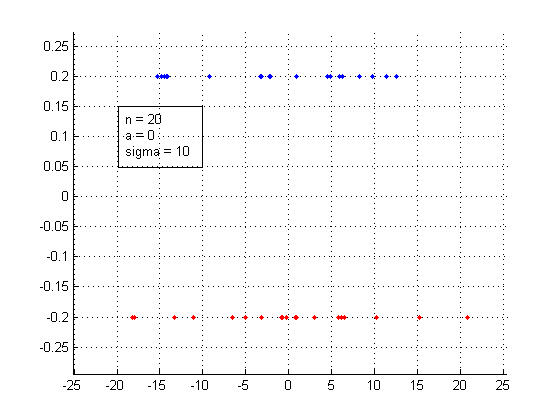
\includegraphics[width=0.9\linewidth]{pic/normal}
  \caption{Случайные величины, распределённые \\ по нормальному закону при заданных параметрах $ a = 0 $, $ \sigma = 10 $}
  \label{pic:normal}
\end{figure}

В верхней части графика находятся значения, полученные с помощью
встроенной функции Matlab. В нижней части --- величины, полученные
с использованием алгоритма, приведенного в подразделе~\ref{sub:theory}.

Статистические оценки параметров выборки:
\begin{align*}
  min (x)  &= -18{,}15, & std (x) = 10{,}07, \\
  max (x)  &= 20{,}83,  & skewness (x) = 0{,}04, \\
  mean (x) &= -0{,}39,  & kurtosis (x) = 2{,}79.
\end{align*}

\newpage

\subsection{Моделирование случайных величин по экспоненциальному закону распределения}

На рисунке~\ref{pic:exp} изображены случайные величины, распределённые
по \textit{экспоненциальному закону}.
\begin{figure}[h!]
  \centering
  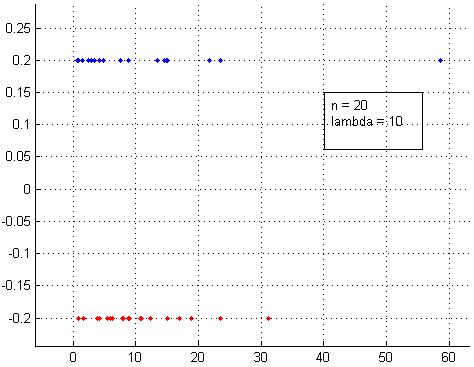
\includegraphics[width=0.9\linewidth]{pic/exp}
  \caption{Случайные величины, распределённые \\ по экспоненциальному закону при заданных параметрах $ \lambda = 10 $}
  \label{pic:exp}
\end{figure}

В верхней части графика находятся величины, полученные с помощью
встроенных функций Matlab, в нижней --- величины, полученные
с использованием алгоритма, приведенного в подразделе~\ref{sub:theory}.

Статистические оценки параметров выборки:
\begin{align*}
  min (x)  &= 0{,}94,  & std (x) = 7{,}63, \\
  max (x)  &= 31{,}15, & skewness (x) = 1{,}21, \\
  mean (x) &= 10{,}30, & kurtosis (x) = 4{,}02.
\end{align*}

\newpage
